
\subsection*{4.2 Sine and Cosine Rules}
The sine and cosine rules are used to find unknown sides and angles in non-right-angled triangles.

\textbf{Key Concepts:}

\begin{center}
	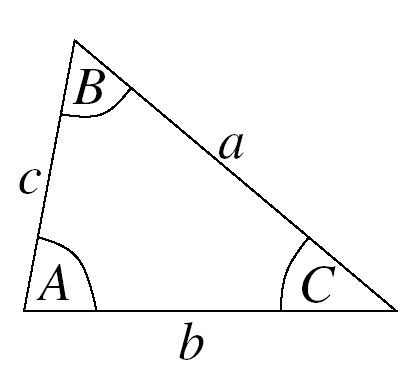
\includegraphics[width=0.6\textwidth]{4.2.png}
\end{center}
\begin{itemize}
	\item \textbf{Sine Rule:} Used when given:
	\begin{itemize}
		\item Two angles and one side (AAS or ASA).
		\item Two sides and a non-included angle (SSA).
	\end{itemize}
	The sine rule states:
	\[
	\frac{a}{\sin A} = \frac{b}{\sin B} = \frac{c}{\sin C},
	\]
	where $a, b, c$ are the sides opposite to angles $A, B, C$ respectively.
	
	\item \textbf{Cosine Rule:} Used when given:
	\begin{itemize}
		\item Two sides and the included angle (SAS).
		\item Three sides (SSS) when finding an angle.
	\end{itemize}
	The cosine rule states:
	\[
	c^2 = a^2 + b^2 - 2ab\cos C.
	\]
	It can also be used to find angles:
	\[
	\cos C = \frac{a^2 + b^2 - c^2}{2ab}.
	\]
	
\end{itemize}

\textbf{Examples:}

\begin{flushleft}
	\textbf{Example 1: Find the length of side $c$ in a triangle where $a = 7$ cm, $b = 9$ cm, and $\angle C = 120^\circ$.}
	
	\vspace{0.5cm}
	\textbf{Solution:}
	\vspace{0.5cm}
	
	Step 1: Use the cosine rule:
	\[
	c^2 = a^2 + b^2 - 2ab\cos C.
	\]
	
	Substituting values:
	\[
	c^2 = 7^2 + 9^2 - 2(7)(9)\cos 120^\circ.
	\]
	
	Since $\cos 120^\circ = -\frac{1}{2}$:
	\[
	c^2 = 49 + 81 - 2(7)(9) \times \left(-\frac{1}{2} \right).
	\]
	
	\[
	c^2 = 49 + 81 + 63 = 193.
	\]
	
	\[
	c = \sqrt{193} \approx 13.9 \text{ cm}.
	\]
	
	Thus, $c \approx 13.9$ cm.
\end{flushleft}

\begin{flushleft}
	\textbf{Example 2: Find angle $B$ in a triangle where $a = 8$ cm, $b = 10$ cm, and $c = 12$ cm.}
	
	\vspace{0.5cm}
	\textbf{Solution:}
	\vspace{0.5cm}
	
	Step 1: Use the cosine rule to find $\cos B$:
	\[
	\cos B = \frac{a^2 + c^2 - b^2}{2ac}.
	\]
	
	Substituting values:
	\[
	\cos B = \frac{8^2 + 12^2 - 10^2}{2(8)(12)}.
	\]
	
	\[
	\cos B = \frac{64 + 144 - 100}{192} = \frac{108}{192}.
	\]
	
	\[
	\cos B = 0.5625.
	\]
	
	Step 2: Find $B$ using inverse cosine:
	\[
	B = \cos^{-1}(0.5625) \approx 55.2^\circ.
	\]
	
	Thus, $\angle B \approx 55.2^\circ$.
\end{flushleft}

\begin{flushleft}
	\textbf{Example 3: Find the missing side $a$ in a triangle where $A = 40^\circ$, $B = 75^\circ$, and $b = 15$ cm.}
	
	\vspace{0.5cm}
	\textbf{Solution:}
	\vspace{0.5cm}
	
	Step 1: Find angle $C$:
	\[
	C = 180^\circ - A - B = 180^\circ - 40^\circ - 75^\circ = 65^\circ.
	\]
	
	Step 2: Use the sine rule:
	\[
	\frac{a}{\sin A} = \frac{b}{\sin B}.
	\]
	
	Substituting values:
	\[
	\frac{a}{\sin 40^\circ} = \frac{15}{\sin 75^\circ}.
	\]
	
	Solving for $a$:
	\[
	a = \frac{15 \times \sin 40^\circ}{\sin 75^\circ}.
	\]
	
	\[
	a \approx \frac{15 \times 0.6428}{0.9659} = \frac{9.642}{0.9659} \approx 9.99 \text{ cm}.
	\]
	
	Thus, $a \approx 10.0$ cm.
\end{flushleft}
